\documentclass{beamer}
\usepackage{amsmath,amssymb,amsfonts}
\usepackage{graphicx}
\usepackage{hyperref}
\usepackage{xcolor}
\usepackage{tcolorbox}
\usepackage{tikz}
\usetheme{Frankfurt} % Elegant theme for a professional look
\usecolortheme{dolphin} % Color theme to give a nice contrast

\title{NCERT 12.9.6.4}
\subtitle{Solving a Differential Equation}
\author{EE24BTECH11036 - Krishna Patil}
\date{\today}

% Define a custom box style for equations
\newtcolorbox[auto counter, number within=section]{mybox}[2][]{colframe=blue!80!black, colback=blue!10, coltitle=black, fonttitle=\bfseries, title=Step #2: #2}

\begin{document}

\frame{\titlepage}

\section{Problem Statement}
\begin{frame}{Problem Statement}
\textbf{Solve the following differential equation:}
\begin{align}
    \frac{dy}{dx} + y \sec x = \tan x
\end{align}
with the initial conditions:
\begin{align}
    x = 0, \quad y = 1.
\end{align}
\end{frame}

\section{Solution Steps}
\begin{frame}{Step 1: Recognize the Linear Form}
The given equation is a first-order linear differential equation of the form:
\begin{equation*}
    \frac{dy}{dx} + P(x)y = Q(x),
\end{equation*}
where
\begin{align*}
    P(x) &= \sec x, \\
    Q(x) &= \tan x.
\end{align*}
\end{frame}

\begin{frame}{Step 2: Find the Integrating Factor}
\begin{mybox}[label={step:integratingfactor}]{Find the Integrating Factor}
The integrating factor (IF) is given by:
\begin{align}
    \mu(x) = e^{\int P(x) dx} = e^{\int \sec x \, dx}.
\end{align}
The integral of $\sec x$ is:
\begin{align}
    \int \sec x \, dx = \ln |\sec x + \tan x|.
\end{align}
Thus, the integrating factor becomes:
\begin{align}
    \mu(x) = \sec x + \tan x.
\end{align}
\end{mybox}
\end{frame}

\begin{frame}{Step 3: Multiply Through by the Integrating Factor}
Multiply the entire differential equation by $\mu(x)$:
\begin{align}
    (\sec x + \tan x) \frac{dy}{dx} + y (\sec x + \tan x) \sec x = (\sec x + \tan x) \tan x.
\end{align}
This simplifies to:
\begin{align}
    \frac{d}{dx} \left( y (\sec x + \tan x) \right) = (\sec x + \tan x) \tan x.
\end{align}
\end{frame}

\begin{frame}{Step 4: Integrate Both Sides}
Integrate both sides:
\begin{align}
    \int \frac{d}{dx} \left( y (\sec x + \tan x) \right) dx = \int (\sec x + \tan x) \tan x \, dx.
\end{align}
The solution to the integral gives:
\begin{align}
    y (\sec x + \tan x) = \sec x + \tan x - x + C,
\end{align}
where $C$ is the constant of integration.
\end{frame}

\begin{frame}{Step 5: Solve for $y$}
Solve for $y$:
\begin{align}
    y = \frac{\sec x + \tan x - x + C}{\sec x + \tan x}.
\end{align}
\end{frame}

\begin{frame}{Step 6: Determine $C$}
Using the initial conditions $x = 0$, $y = 1$:
\begin{align}
    1 = \frac{\sec 0 + \tan 0 - 0 + C}{\sec 0 + \tan 0}.
\end{align}
This simplifies to:
\begin{align}
    1 = 1 + C \implies C = 0.
\end{align}
Thus, the solution is:
\begin{align}
    y = \frac{\sec x + \tan x - x}{\sec x + \tan x}.
\end{align}
\end{frame}

\section{Numerical Solution}
\begin{frame}{Step 7: Numerical Solution}
For a numerical solution, we use the iterative logic:
\begin{align}
    x_0 &= 0, \quad y_0 = 1, \quad h = 0.001, \\
    y_{n+1} &= y_n + h \cdot (\tan x_n - y_n \sec x_n), \\
    x_{n+1} &= x_n + h.
\end{align}
\end{frame}

\section{Verification}
\begin{frame}{Verification}
Below is a graph verifying the solution:
\begin{figure}[h]
    \centering
    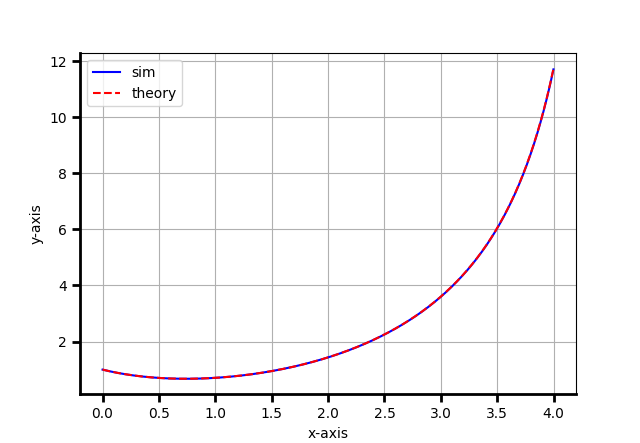
\includegraphics[width=0.8\columnwidth]{fig/Figure_1.png}
    \caption{Graphical Verification of the Solution}
\end{figure}
\end{frame}

\end{document}


